\documentclass{article}
\papersize{a4}
\usepackage{pgf}
\usepackage{float}
\usepackage{tikz}
\usepackage{caption}
\usepackage{lipsum}
%!\usetikzlibrary;
\begin{document}

\begin{flushleft}
Freie Universität Berlin\\
Institut für Deutsche und Niederländische Philologie\\

% Zeit\\
% Raum\\
Wintersemester 2022/23
\end{flushleft}

\vspace{0.2cm}

\begin{center}
\LARGE{Phrasenschemata}\\[10pt]
\Large{Themenblatt}\\[10pt]
\large{XXXX name}\\[3pt]
\small{\pgfrdfhref{mailto:x@xtdialup.fu-berlin.de}{noadressfu-berlin.de}}\\[10pt]
\large{\today}\\[30pt]
\end{center}


\section{essai}
1st line\\[14pt]

\begin{figure}[h]\label{figure1}
\centering

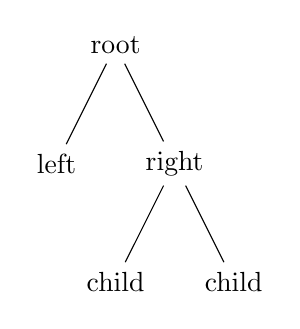
\begin{tikzpicture}
\node {root} 
child {node {left}} 
child {node {right} 
child {node {child}} 
child {node {child}}};
%!\caption{this is a figure}
%!\label{figure1}
  \end{tikzpicture}
  \caption{A picture}
  \end{figure}
\end{document}

blub undsoweiter
for reference see: \cref{figure1}